
As established in the methodology, the top boundary of the lane (the pin deck interface) presents a unique geometric challenge: the physical edge is heavily occluded by the bowling pins themselves, making standard gradient-based edge detection ineffective. To overcome this occlusion, feature-based object detection methods, specifically SIFT, were initially evaluated for pin localization. While SIFT is generally highly robust to scale and rotation variations, it proved ineffective in this specific environment. The primary limitation arises from the small relative size of the pins within the global image frame at typical camera distances. Furthermore, because bowling pins possess a smooth, uniform surface with minimal internal texture, they generate an insufficient number of stable, high-contrast keypoints. Qualitative analysis of the feature matching outputs (see Figure \ref{fig:sift_failure}) revealed that the algorithm consistently failed to localize the target pins on the deck. Instead, the limited keypoints extracted from the pin template produced spurious, incorrect matches with high-frequency noise and visually complex elements in the background, such as wall graphics. Due to this inability to reliably detect the target objects, feature-based extraction was discarded in favor of the intensity-based template matching approach, which successfully leverages the macro-structural silhouette of the pins rather than internal textural features.

% --- FIGURE FOR SIFT FAILURE ---
\begin{figure}[htbp]
    \centering
    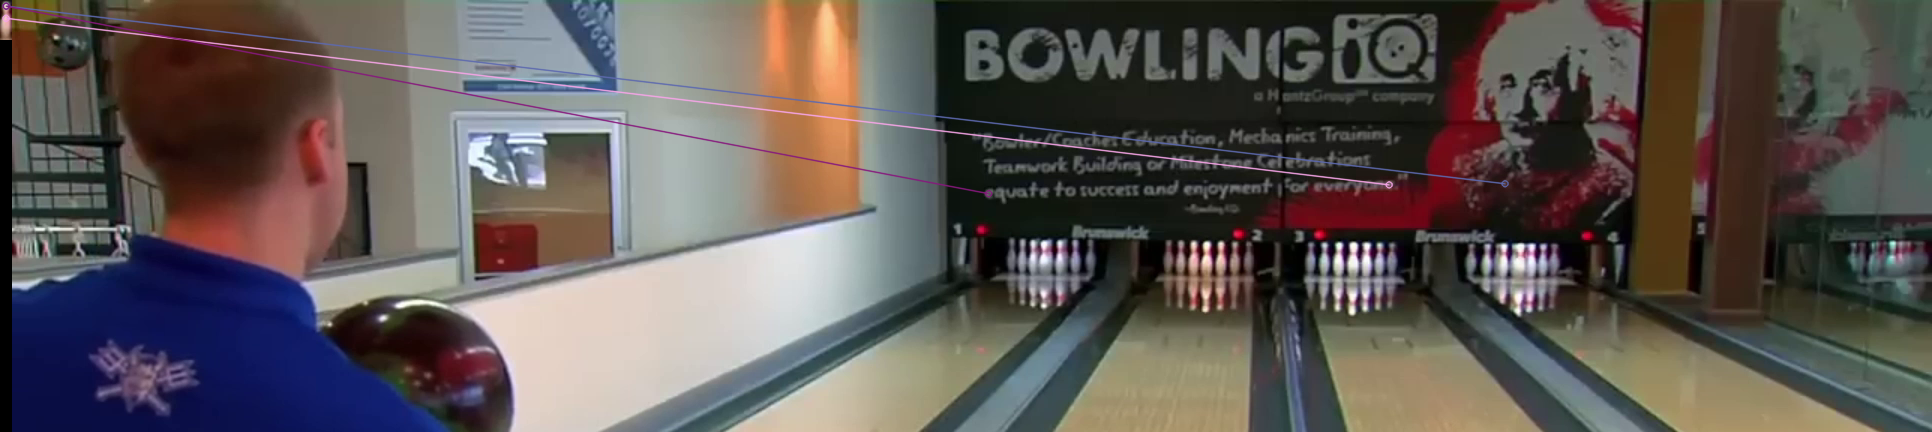
\includegraphics[width=0.9\textwidth]{figures/results/sift_matches.png}
    \caption{Failure of SIFT feature matching for pin detection. Due to the small scale and lack of internal texture on the pins, the algorithm fails to find valid corresponding keypoints on the pin deck. Instead, it generates spurious matches between the template (top left) and random high-frequency background elements.}
    \label{fig:sift_failure}
\end{figure}

For this reason, the pipeline employs multi-scale template matching to isolate the pins, extracting the bottom-center coordinates of their resulting bounding boxes as spatial candidate points for the boundary (see Figure \ref{fig:template_bboxes}). 

The specific selection of the bottom-center coordinate, rather than the geometric centroid (midpoint) of the bounding box, is a critical design choice. Empirical analysis of the bounding box outputs revealed that using the centroid artificially elevated the regression line, mapping it across the midsections of the pins rather than the lane surface (Figure \ref{fig:midpoint_vs_bottom}, Top Row). Because the physical objective is to map the pin deck interface, the bottom-center coordinate provides a geometrically accurate anchor directly to the true floor plane (Figure \ref{fig:midpoint_vs_bottom}, Bottom Row).

\begin{figure}[htbp]
    \centering
    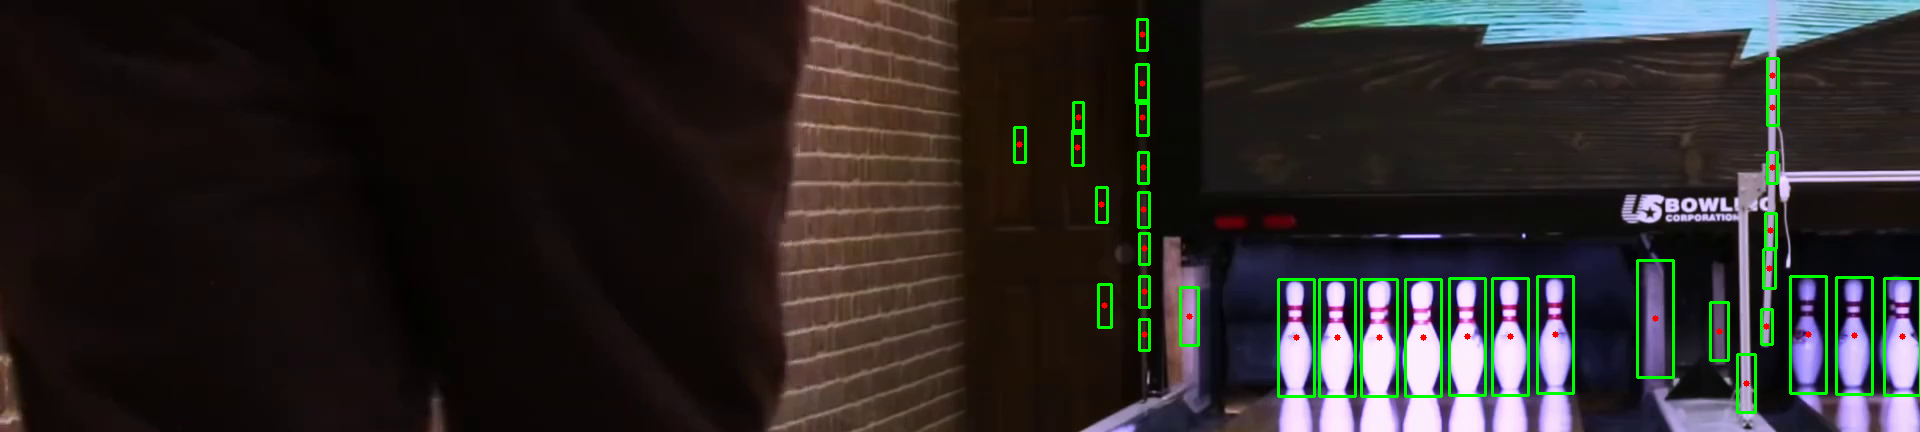
\includegraphics[width=0.9\textwidth]{figures/results/template_matches.png}
    \caption{Multi-scale template matching detections. The algorithm draws bounding boxes around identified bowling pins, capturing structural silhouettes on the target pin deck, adjacent lanes, and occasional background false positives.}
    \label{fig:template_bboxes}
\end{figure}

\begin{figure}[htbp]
    \centering
    % Top Pair: Midpoint / Centroid Estimation
    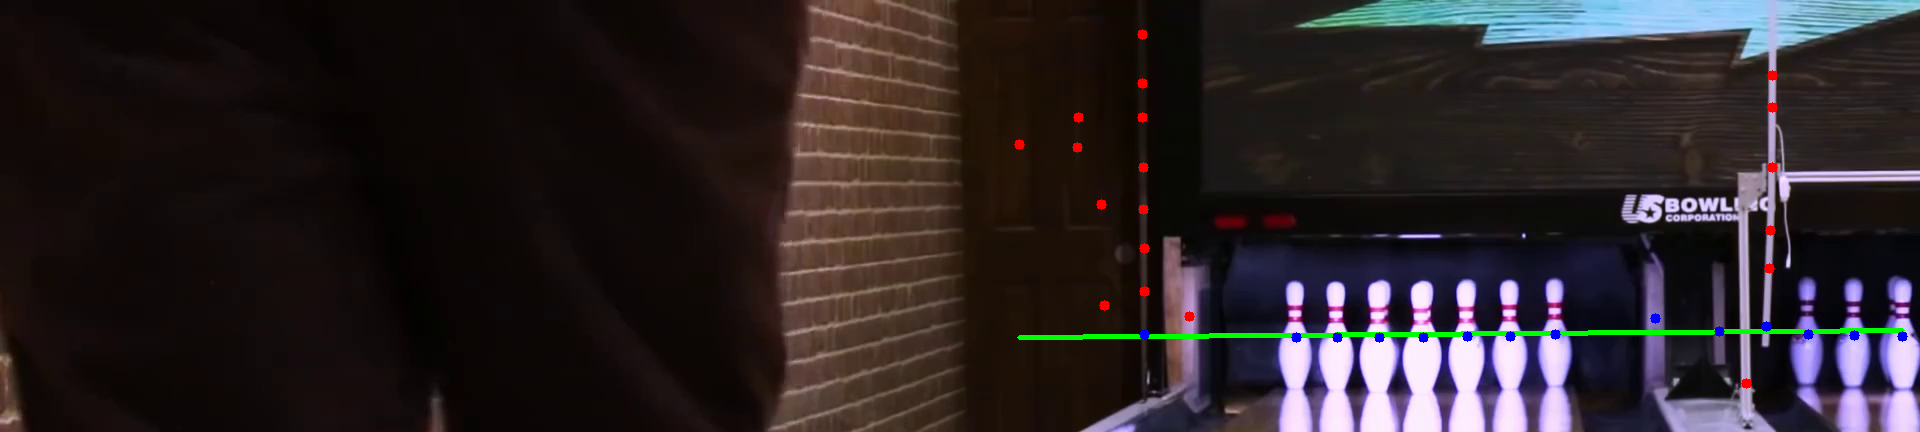
\includegraphics[width=0.48\textwidth]{figures/results/top_boundary_clip4_center.png}
    \hfill
    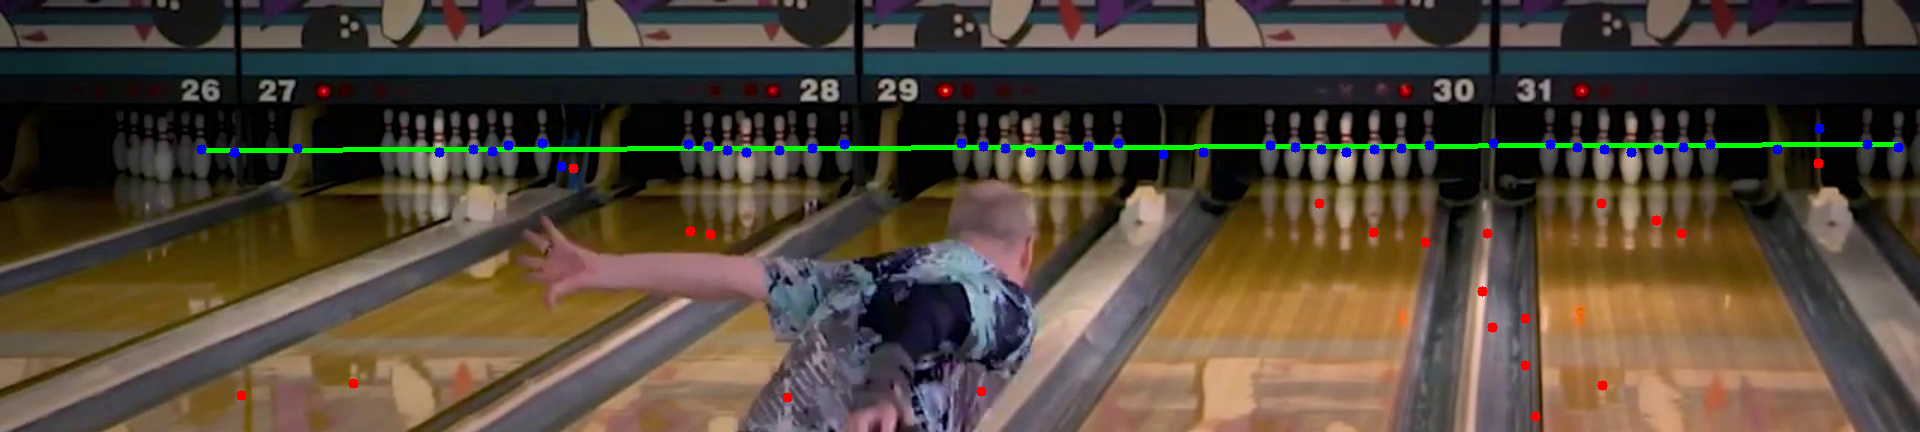
\includegraphics[width=0.48\textwidth]{figures/results/top_boundary_clip2_center.png} 
    
    \vspace{0.2cm}
    
    % Bottom Pair: Bottom-Center Estimation
    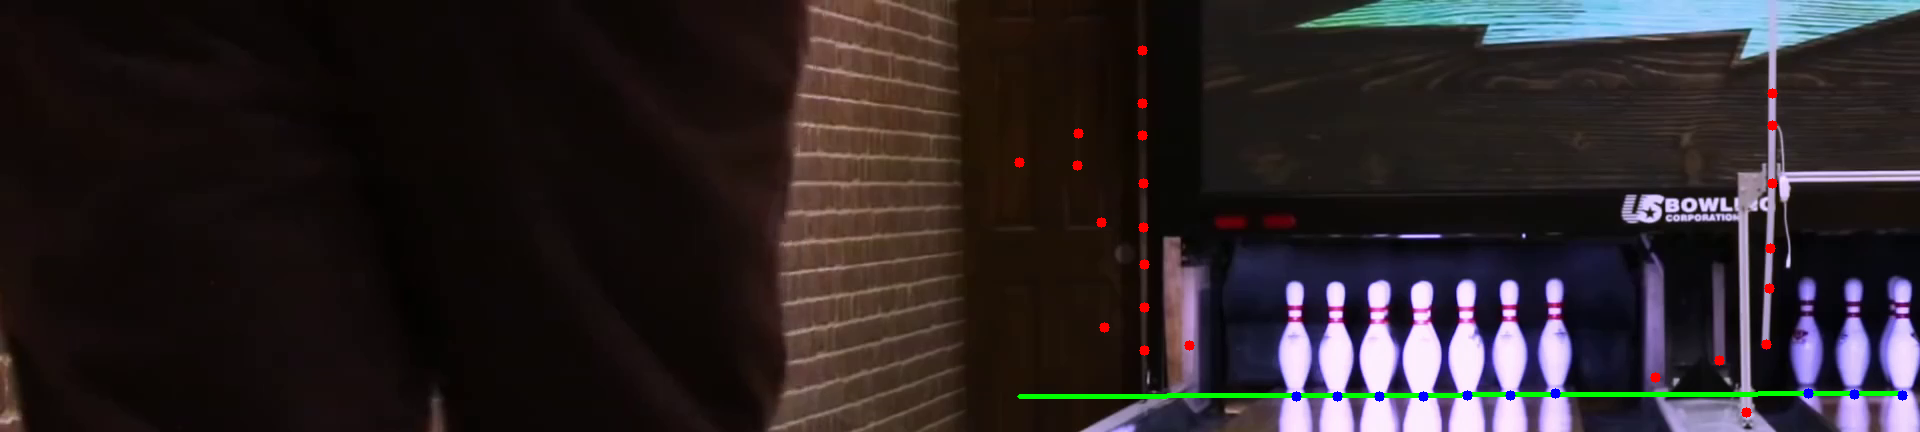
\includegraphics[width=0.48\textwidth]{figures/results/top_boundary_clip4_bottom.png}
    \hfill
    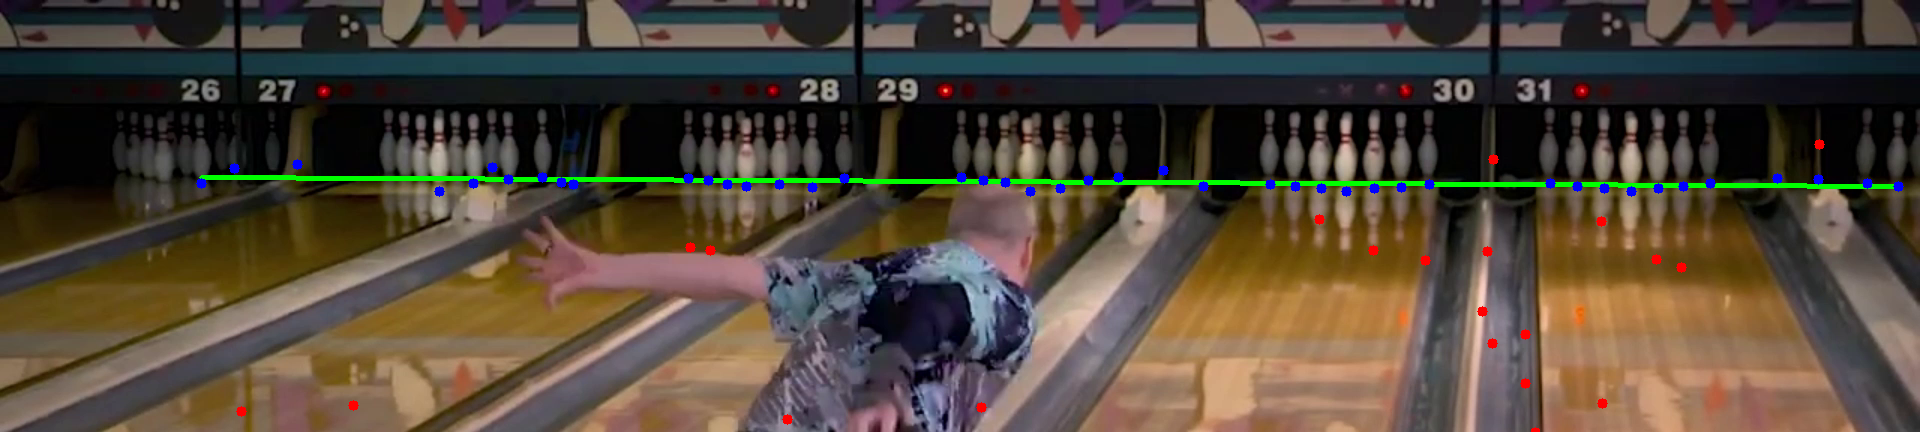
\includegraphics[width=0.48\textwidth]{figures/results/top_boundary_clip2_bottom.png}
    
    \caption{Comparison of boundary candidate coordinate selection. Top Row: Utilizing the bounding box centroids (midpoints) artificially elevates the regression line, mapping it across the "necks" of the pins. Bottom Row: Utilizing the bottom-center coordinates correctly anchors the estimated regression line to the true floor plane at the pin deck interface.}
    \label{fig:midpoint_vs_bottom}
\end{figure}


While multi-scale template matching successfully localized the target pins, the raw output was inherently noisy. As anticipated in a visually complex bowling environment, the algorithm frequently generated false positive detections, predominantly from pin reflections on the highly polished synthetic oil and visually similar architectural features in the background. Interestingly, the template matching also frequently detected pins actively standing in adjacent parallel lanes. Rather than treating these adjacent detections as noise, the pipeline exploits them to increase the stability of the boundary estimation. Because bowling alleys are constructed with coplanar, horizontally aligned pin decks, pins in adjacent lanes share the exact same geometric baseline as the target lane. Consequently, these adjacent detections serve as valid, extended data points that drastically improve the stability of the linear estimation.

To robustly extract the true boundary from this spatial data while filtering out the actual noise, a RANSAC regressor was evaluated. RANSAC is uniquely suited for this task due to its outlier rejection capabilities. By iteratively estimating a first-degree polynomial model from random subsets of the spatial coordinates, the algorithm successfully identified the dominant linear structure (the continuous base of the pins extending across the visible lanes) while ignoring coordinate data from reflections and background architecture that did not conform to this geometry.

Qualitative analysis of the regression output (see Figure \ref{fig:ransac_pin_deck}) demonstrates the high efficacy of this approach. The RANSAC algorithm successfully segmented the raw candidate points into an inlier consensus set (visualized as blue points) and a rejected outlier set (visualized as red points). The inlier set actively incorporates valid pins from both the target and adjacent lanes, exploiting the extended horizontal baseline to correctly estimate the top boundary. The red spatial outliers encapsulate the false detections caused by reflections and background noise. By fitting the final line to these blue inliers, the pipeline generated an accurate and stable top boundary line (visualized in green). This confirms that decoupling the structural detection into an object-centric model effectively bypasses severe visual occlusions at the pin deck. 




% --- FIGURE FOR RANSAC ---
\begin{figure}[htbp]
    \centering
    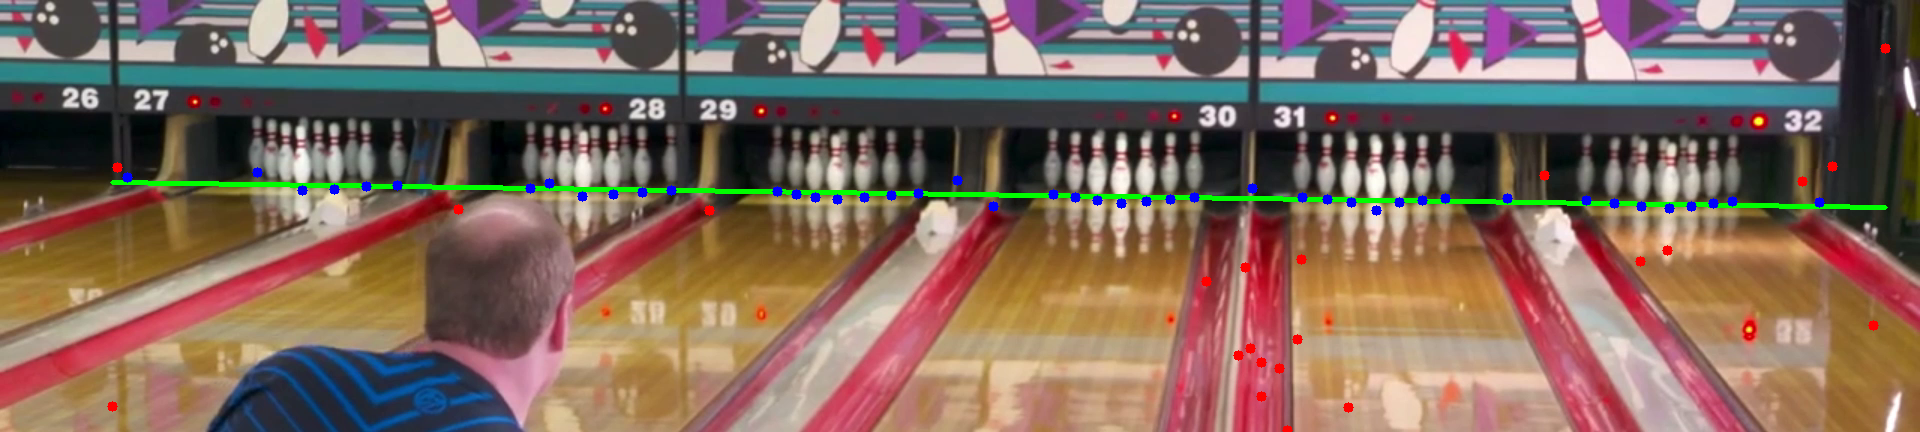
\includegraphics[width=0.9\textwidth]{figures/results/top_boundary_ransac.png}
    \caption{Performance of the RANSAC regressor on multi-scale template matching output. The bottom-center coordinates of all detected bounding boxes are plotted. The algorithm successfully classifies true pins (including those on adjacent, aligned lanes) as inliers (blue dots). It effectively rejects false positives from reflections and background structures as outliers (red dots). The final fitted polynomial (green line) accurately maps the occluded pin deck boundary using the extended geometric baseline.}
    \label{fig:ransac_pin_deck}
\end{figure}
